\section{OpenFace im Test}
Da mit diesem Verfahren die Landmarks bestimmt werden, aus denen die Gesichtsorientierung abgeleitet wird, sollen die Grenzen dieses Verfahrens ermittelt werden. Von Interesse ist die Bildqualität in der ein Gesicht dargestellt werden muss um dieses noch verarbeiten zu können und wie sehr diese Person von der Kamera abgewandt sein kann.\\
Das Herunterskalieren von Bildern ist nicht das selbe wie eine Aufnahme auf großer Distanz, ist aber ähnlich genug um eine Aussage darüber treffen zu können.
\subsection{Auswirkung der Auflösung auf die Detektionsrate}
Durch die Aufgabenstellung muss das Verfahren zuverlässig bezüglich der Distanzen bzw. Darstellungsgröße sein. Zur Messung wurde der Datensatz von Labeled Faces in the Wild \cite{database_Face} verwendet. Dieser Bilddatensatz enthält Abbildungen verschiedener Personen mit einer durchschnittlichen Abbildung der Breite des Kopf von 94 Pixeln. Bei Random Forests for Real Time 3D Face Analysis \cite{database_Face_Ori} beträgt die durchschnittliche Breite 78 Pixel.\\
Um die Grenzen der Methode auszuloten wurde das Bild mit unterschiedlichen Faktoren linear skaliert, um so weiter entferntere Gesichter zu simulieren.\\
Um die Detektionsrate zu bestimmen, wurde der Image-Detector von OpenFace auf den skalierten Bildern angewendet und gezählt wie oft der Detektor ein Gesicht erkannt hat. Dabei wurde nicht geprüft ob des sich dabei um ein korrektes Gesicht handelt.\\
Das Ergebnis dieser Messung ist in \autoref{img_lineareverkleinerung} dargestellt. Es ist zu erkennen, dass die Wahrscheinlichkeit einer erfolgreichen Detektion ab einer Skalierung von $0,6$ bei BIWI (Gesichert mit etwa 47 Pixel Breite) rapide abnimmt. Bei der in \autoref{hardware} beschriebenen Kamera entspricht dies einer Distanz von etwa $4,5m$.\\
\begin{figure}
	\centering
	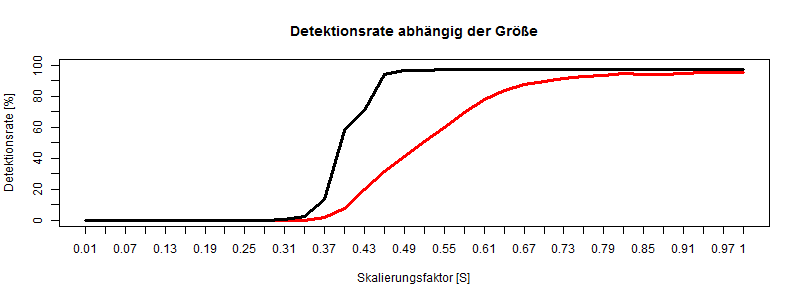
\includegraphics[width=\linewidth]{img_Skalierung/Gesicht_Rate}
	\caption{Die Bilder aus Labeled Faces in the Wild \cite{database_Face} (schwarz) und Biwi Kinect Head Pose Database \cite{BIWI_database} (grau) wurden mit den Faktor auf der X-Achse linear verkleinert und die Erkennungsrate Y-Achse abgebildet}
	\label{img_lineareverkleinerung}
\end{figure}
\subsection{Auswirkung der verschiedenen Skalierungesverfahren auf die Detektion}
\label{OpenFace_skal}
Um die Auswirkung der Skalierungsverfahren zu bestimmen, wurden verschiedene Gesichtsgrößen simuliert, indem sie um den angegeben Faktor linear verkleinert wurden.\\
Beim Random Forest Datensatz \cite{database_Face_Ori} werden nur jene Bilder ausgewertet, in denen OpenFace bei einem Vorabtest ein Gesicht erkannte und nur der entsprechende Bildbereich ausgewertet. Als Zielgröße bei der Skalierung wurde das $1,3\times$ der Originalgröße gesetzt, damit die abgebildeten Gesichter in etwa 100 Pixel groß sind.\\
Bei dem Labeled Faces in the Wild \cite{database_Face} Datensatz wurden alle Bilder im Orginal verwendet, um den angegebenen Skalierungsfaktor verkleinert und mit dem angegebenen Verfahren wieder auf die Orginalgröße gebracht.\\
Die Auswirkung der verschiedenen Skalierungsverfahren auf die Detektionswahrscheinlichkeit ist in \autoref{img_hochskalliern} dargestellt. Dabei wurden die Bilder linear um den angegebene Faktor verkleinert und mittels der verschieden Verfahren wieder vergrößert.\\
Es ist zu erkennen, dass die Detektionsrate über einen weiten Bereich, $[1;0,25]$ bei der Skalierung, nur sehr wenig abnimmt. Durch die Vergrößerung können somit jene Gesichter in Skalierungsbereichen ausgewertet werden, die ohne nicht erkennbar sind.\\
Erst bei den sehr kleinen Skalierungen ist ein wirklicher Unterschied zwischen den Verfahren zu erkennen. So nimmt die Detektionsrate bei  Nearest-Neighbor (rot) deutlich früher ab als bei den anderen Verfahren. Das Bicubic (blau) und Lanczos (grün) Verfahren haben die höchste Detektionsrate und fallen zuletzt ab, wobei Bicubic minimal besser ausfällt.\\
Durch diesen Test kann nachgewiesen werden, das durch die Skalierung die Anforderungen auf eine Detektion von Gesichtern mit 22 Pixel (Skalierung $0,25$, $8m$) erfüllt werden kann. Theoretisch wären sogar Distanzen bis zu $14m$ möglich (basierend auf der hohen Auflösung der Actioncam).
\begin{figure}
	\centering
	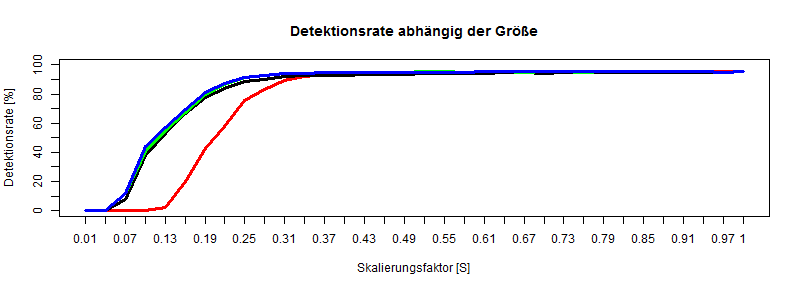
\includegraphics[width=\linewidth]{img_Skalierung/Resize_Rate_Ges}\\
	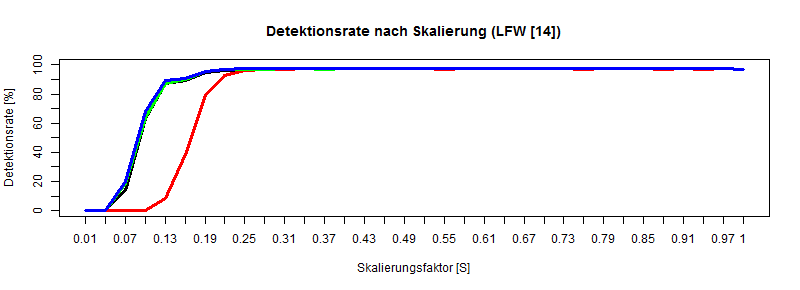
\includegraphics[width=\linewidth]{img_Skalierung/Resize_Rate_lfw}
	\caption{Die Bilder wurden mit den Faktor auf der X-Achse linear verkleinert und mit den verschiedenen Verfahren wieder vergrößert.\\
		Bicubic (blau), Lanczos (grün), Linear (schwarz), Nearest-Neighbor (rot)}
	\label{img_hochskalliern}
\end{figure}
\subsection{Auswirkung der verschiedenen Skalierungesverfahren auf den Arbeitsbereich bezüglich Rotation}
In \autoref{img_Rot_Dif} ist der Median der Differenz zwischen per OpenFace berechnetem und im Datensatz angegebenem Kopforientierungswinkel aufgetragen.\\
Bei der X-Rotation zeigt sich, dass das Bicubic-Verfahren im Vergleich zu den anderen 1 Grad schlechter abschneidet. Der Fehler von Lanczos, Linear und Nearest-Neighbor liegt bei etwa $19^\circ$ bis zu einer Skalierung von $0,25$.\\
Der Median der Fehler auf der Y-Achse (nicken) sehr hoch ausfällt mit knapp über $25^\circ$. 
Dabei liefern alle vier Verfahren nahezu identische Ergebnisse, die auch konstant bleiben bezüglich der Skalierung.\\
Die Z-Rotation wird am besten bestimmt mit einer Abweichung von etwa $7,5^\circ$, dabei ist aber auch zu beachten, das der Wertebereich deutlich geringer ausfällt im Datensatz, als bei den anderen beiden Rotationen. Für diese Rotation liefert Bicubic das beste Ergebnis, wobei der Unterschied weniger als ein halbes Grad beträgt.\\
Für alle Berechnungen zeigt sich, das der Fehler konstant bleibt, bis zu der Skalierung von $0.25$, bei der auch die Detektion scheitert.\\
Neben der Qualität der bestimmten Winkel, ist auch der Arbeitsbereich von Interesse in dem Gesichter bei verschiedenen Skalierungen noch erkannt werden können, da ein Gesicht das außerhalb dieser Bereiche liegt nicht erkannt und ausgewertet werden kann.\\
In \autoref{img_Rot_Max} sind die Quantile bei $50\%; 80\%; 99,5\%$ und der Maximalwert, von den Rotationswinkel der Bilder aus dem Biwi Kinect Head Pose Database \cite{BIWI_database} ein Gesicht erkannt wurde, abgebildet. Durch den großen Unterschied zwischen dem $80\%$-Wert, $99,5\%$-Wert und dem Maximalwert liegt die Vermutung nahe, dass es sich bei diesen Werten um falsch detektierte Bilder handelt, aber eine Rotation des Kopfes von $45\%$ in alle Richtungen erkannt und ausgewertet werden kann.\\
Eine genaue Darstellung der Messung ist in \autoref{Abbildungen} abgebildet, für die X-Rotation \autoref{img_X_Rot_Skal}, Y-Rotation \autoref{img_Y_Rot_Skal} und Z-Rotation \autoref{img_Z_Rot_Skal}.
\begin{figure}
	\centering
	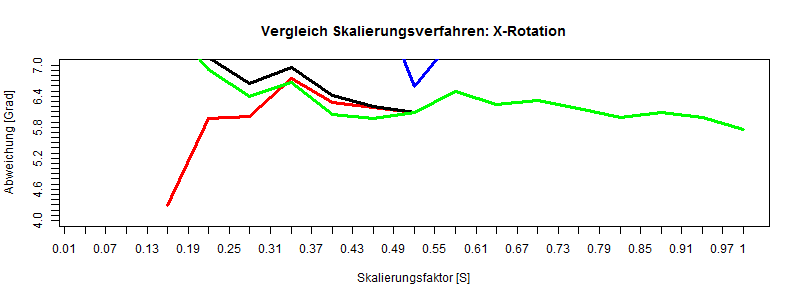
\includegraphics[width=\linewidth]{img_Skalierung/Skal_Diff_RX}
	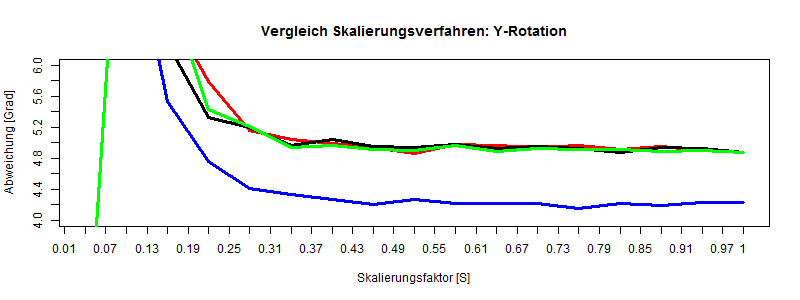
\includegraphics[width=\linewidth]{img_Skalierung/Skal_Diff_RY}
	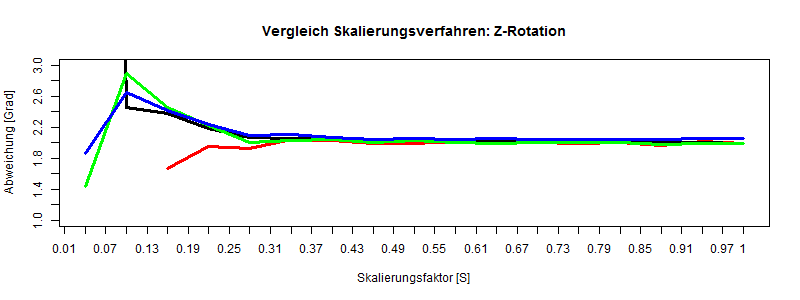
\includegraphics[width=\linewidth]{img_Skalierung/Skal_Diff_RZ}
	\caption{Dargestellt ist der Median der Abweichung zwischen der Berechneten Drehung und der des Datensatzes.\\
		Bicubic (blau), Lanczos (grün), Linear (schwarz), Nearest-Neighbor (rot)}
	\label{img_Rot_Dif}
\end{figure}
\subsection{Auswirkung der Skalierungsverfahren auf die Positionsbestimmung}
Für eine zuverlässige Auswertung ist auch die Bestimmung der Position von Interesse. Im Biwi Kinect Head Pose Database \cite{BIWI_database} ist die durchschnittliche Distanz zwischen Kamera und Proband etwa $90cm$. Zur Berechnungen der Position wurde eine Brennweite der Kinekt-Kamera auf $531,15$ geschätzt, da es keine Angabe für den Datensatz gibt. Der Median der Differenz zwischen Datensatz und Rechnung ist in \autoref{img_Pos_Dif} dargestellt. Bei sehr kleinen Skalierungen existieren durchaus auch sehr große Fehler, diese wurden allerdings bei der Darstellung abgeschnitten, da bei dieser Größe die Detektionsrate so klein ist, dass sie nahezu irrelevant werden.\\
Es zeigt sich, das die Position in horizontaler und vertikaler Richtung auf etwa $6,5cm$ genau bestimmt werden kann, die Distanz (Tiefe) auf $9cm$ genau, selbst bei sehr klein skalierten Bildern.\\
Nearest-Neighbor hat bei der Berechnung der X-Position die geringste Abweichung zu den anderen getesteten Verfahren mit $6,37cm$ bei der Originalgröße.\\
Bei der Bestimmung der Y-Position, liefern alle Skalierungsverfahren sehr ähnlich Ergebnisse mit einem Fehler von $6,5cm$, wobei das lineare Verfahren minimal besser ausfällt bei kleinen Skalierungen.\\
Die größte Ungenauigkeit liegt bei der Z-Position (Tiefe). Das Lineare Verfahren liefert auch hier das beste Ergebnis, mit einer Abweichung von $8,92cm$, dabei ist der Unterschied zu den anderen Verfahren minimal.\\
Eine ausführliche Darstellung der Messung ist in \autoref{img_X_Pos_Skal}, \autoref{img_Y_Pos_Skal} und \autoref{img_Z_Pos_Skal} dargestellt.
\begin{figure}
	\centering
	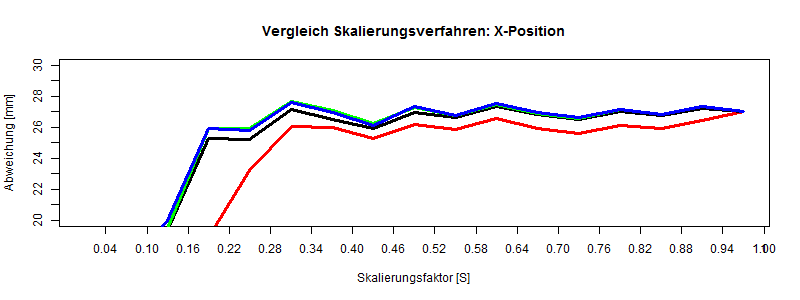
\includegraphics[width=\linewidth]{img_Skalierung/Skal_Diff_TX}
	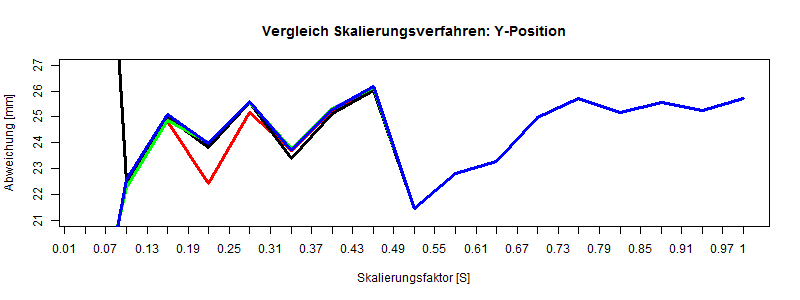
\includegraphics[width=\linewidth]{img_Skalierung/Skal_Diff_TY}
	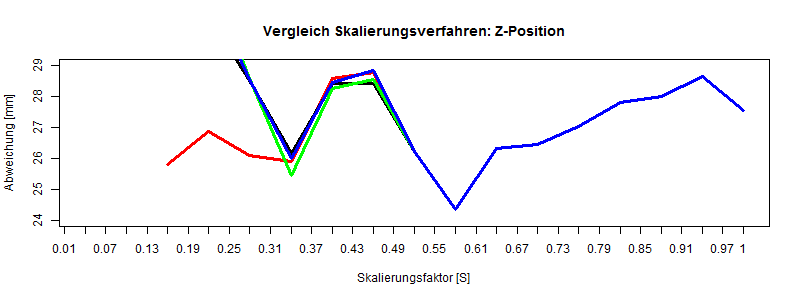
\includegraphics[width=\linewidth]{img_Skalierung/Skal_Diff_TZ}
	\caption{Dargestellt ist der Median der Abweichung zwischen der Berechneten Drehung und der des Datensatzes.\\
		Bicubic (blau), Lanczos (grün), Linear (schwarz), Nearest-Neighbor (rot)}
	\label{img_Pos_Dif}
\end{figure}
\subsection{Auswirkung von Pixelrauschen auf die Detektion}
Mit diesem Test soll geprüft werden, welches der Verfahren auch stabil gegenüber Rauschen ist.\\
Um Pixelrauschen zu simulieren, wurden die Bilder aus Labeled Faces in the Wild \cite{database_Face} entsprechend verkleinert, mit Rauschen versehen um sie anschließend mit den unterschiedlichen Verfahren zu vergrößern.\\
Das Rauschen wird für jedes Pixel simuliert, indem eine Wahrscheinlichkeit von $50\%$ besteht auf eine gleich verteilte Abweichung von $\pm 10\%$ des originalen Farbwertes. Dieser Vorgang wurde für jedes Bild viermal wiederholt um Zufälligkeiten bei der Rauschsimulation zu vermeiden.\\
Wie zu erwarten ist Nearest-Neighbor am schlechtesten, aber auch zwischen den anderen Verfahren sind nun Unterschiede zu erkennen, siehe \autoref{img_hochskalliern_nois}. Die gesamte Erkennungsrate ist signifikant kleiner als ohne Rauschen, wobei die Position $(0.15)$, ab welcher die Erkennungsrate rapide abfällt, beibehalten wird.
\begin{figure}
	\centering
	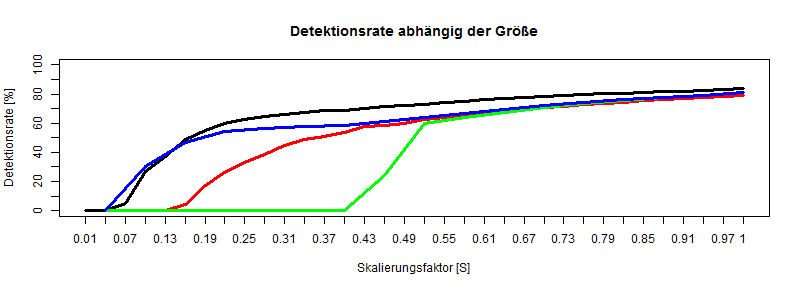
\includegraphics[width=\linewidth]{img_Skalierung/Hochskalliern_Nois}
	\caption{Bilder aus Labeled Faces in the Wild \cite{database_Face}, mit dem X-Faktor verkleinert, um jedes Pixel mit $50\%$ Wahrscheinlichkeit auf $\pm 10\%$ Gleichverteilung der Abweichung}
	\label{img_hochskalliern_nois}
\end{figure}
\subsection{Ergebnis bezüglich Verwendbarkeit}
Für die Anwendung werden die Bildbereiche der Gesichter mit MTCNN-Face bestimmt, allerdings müssen die Bereiche nicht exakt sein, da OpenFace einen eigenen Facedetector besitzt. Je nach verwendetem Trainingsdatensatz und darin enthaltener Annotation werden z.B. Kinn und Haaransatz noch als Gesichtsbereich oder schon als außerhalb betrachtet. So geben beiden Methoden (OpenFace und MTCNN-Face) Boxen aus, diese sind in ihren Ausmaßen allerdings nicht identisch. Da die folgende Verarbeitung eine OpenFace-skalierte Box erwartet, hat sich eine Vergrößerung der MTCNN-Face Box um $30\%$ als sinnvoll erwiesen, um Ungenauigkeiten bezüglich der Position und Dimension des Kopfes im Bild entgegen zu wirken.\\
Anhand der Detektionsrate abhängig von der Skalierung, siehe \autoref{img_lineareverkleinerung}, kann entnommen werden, das Gesichter unter 50 Pixel Größe nicht mehr sinnvoll erkannt werden können. Somit ergibt sich eine maximale Distanz von etwa $4,5m$ (basierend auf der Actioncam) für eine Analyse.\\
Werden die Bildbereiche hingegen hochskaliert, können sogar Gesichter mit einer Größe von 25 Pixel gefunden werden. Dies bedeutet, dass mit diesem Trick auch mit der Hälfte des Informationsgehaltes noch gearbeitet werden kann, wenn sie dadurch dem Trainingsdatensatz eher entsprechen.\\
Für eine erfolgreiche Analyse sind die Parameter Detektionsrate, Qualität der Rotation und Qualität der Position relevant. Daher wurden die verschiedenen Skalierungsverfahren in diesen Parametern bei unterschiedlichen Größen der Eingabebilder verglichen.\\
Die höchste Detektionsrate bei den Skalierungen erreicht Bicubic, wobei der Unterschied zu Lanczos und Linear so minimal ausfällt, das sie als Gleichwertig in diesem Bereich betrachtet werden kann. Es Zeigt sich auch die deutliche Schwäche von Nearest-Neighbor, die Detektionsraten nimmt deutlich früher ab als bei den anderen.\\
Bei der Bestimmung der Rotation kann nur ein geringer Unterschied zwischen den einzelnen Verfahren erkannt werden. Für die X-Rotation hat das Bicubic-Verfahren einen um etwa $1,5^\circ$ größeren Fehler als die anderen. Bei der Y-Rotation liegen alle Verfahren so nahe beieinander, das sie als gleich gut betrachtet werden können. Bei der Z-Rotation ist Bicubic hingegen um $0,5^\circ$ genauer als die anderen Drei. Somit ist bei diesem Parameter die Wahl des Verfahrens egal.\\
Zur Bestimmung der Position ist das lineare Verfahren am besten geeignet, da es den kleinsten Fehler aufweist, wobei der Unterschied mit $0,5mm$ sehr gering ausfällt.\\
Der Test mit dem Pixelrauschen soll etwaige Bildfehler simulieren, wie es bei schlechten Kameras der Fall sein kann, was die Auswertung auf kleinen Bildausschnitten erschwert. Somit kann auch gezeigt werden, dass dieser Trick mit der Vergrößerung auch sehr wahrscheinlich in der späteren Anwendung funktionieren wird. In diesem Test erreicht das lineare Verfahren die höchste Detektionsrate, diesmal ist der unterschied zwischen den einzelnen Verfahren deutlich besser erkennbar.\\
Somit erfüllt das linear Verfahren die Parameter am besten, wobei der Unterschiede zwischen den einzelnen recht gering ausfällt und die Wahl des Skalierungsverfahren durch andere Kriterien abhängig gemacht werden wie z.B. der Rechenzeit. Dabei kann vom Nearest-Neighbor abgeraten werden wegen der deutlich früherem Abfall der Detektionsrate.